\documentclass{article}
\usepackage[utf8]{inputenc}
\usepackage{amsmath} 
\usepackage{amsthm}
\usepackage[margin=1in]{geometry}
\usepackage{graphicx}
\usepackage{float}
\setlength\parindent{0pt}

\newtheorem*{definition}{Definition}
\newtheorem*{theorem}{Theorem}


\begin{document}

\section*{Construct a graph}
Construct a simple graph, \(G = (V, E)\), such that:

\begin{align}
|V| &\geq 8 \\
\chi(G) &> \chi^{*}(G)
\end{align}

Let \(\chi\) refer to the coloring generated by using the greedy algorithm with degree sequencing heuristic. Let \(\chi^{*}\) be the optimal coloring.

\subsection*{Example 1}
I constructed a simple graph, \(G = (V, E)\), such that \(\Delta(G) = 3\) and \(\delta(G) = 1\). I've let \(|V| = 8\) for this example.

\begin{figure}[H]
\centering
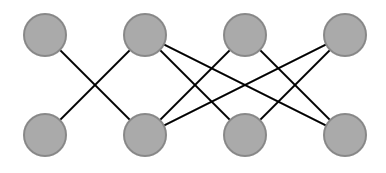
\includegraphics[scale=0.5]{graph-1.png}
\caption{Uncolored original graph \(G\)}
\end{figure}

By applying the greedy algorithm plus degree sequencing heuristic, we get the following coloring. The numbers indicate the ordering of vertices before applying the greedy algorithm. Any vertex of the same degree got assigned arbitrarily. This results in \(\chi(G) = 3\).

\begin{figure}[H]
\centering
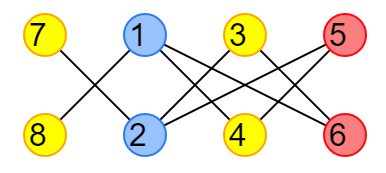
\includegraphics[scale=0.5]{graph-2.png}
\caption{Coloring from applying the greedy plus degree sequencing heuristic}
\end{figure}

We can see that this is a bipartite graph and thus is \emph{2-colorable}. This means \(\chi^{*}(G) = 2\). Thus, this is an example graph that satisfies conditions \((1)\) and \((2)\). The optimal coloring is shown below.

\begin{figure}[H]
\centering
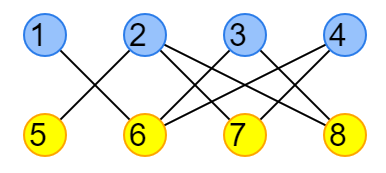
\includegraphics[scale=0.5]{graph-3.png}
\caption{Optimal coloring of graph \(G\)}
\end{figure}

\newpage

\section*{Upper Bounds}
Examine the upper bounds of the greedy heuristic and the greedy plus degree sequencing heuristic. \newline

To do so, let's create another example that satisfies conditions \((1)\) and \((2)\) from above. After doing some research into bipartite graphs, I learned that \emph{crown graphs} are excellent at showing how bad greedy heuristics can be.

\begin{definition}[Crown Graph]
A crown graph is a complete bipartite graph where the edges of a perfect matching have been removed.
\end{definition}

\subsection*{Example 2}

I constructed a simple crown graph, \(H = (V, E)\). I've let \(|V| = 10\) for this example.

\begin{figure}[H]
\centering
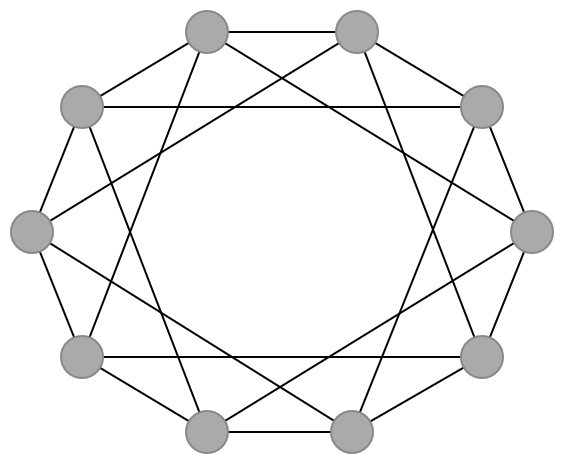
\includegraphics[scale=0.40]{graph-4.png}
\caption{Uncolored original graph \(H\)}
\end{figure}

We can see that \(\Delta(G) = 4\). We can also see \(d(v) = 4\) for all \(v \in V\). Thus, in both heuristics, the greedy algorithm would pick an order arbitrarily. We can show using this crown graph the worst-case scenario of these heuristics.

\begin{figure}[H]
\centering
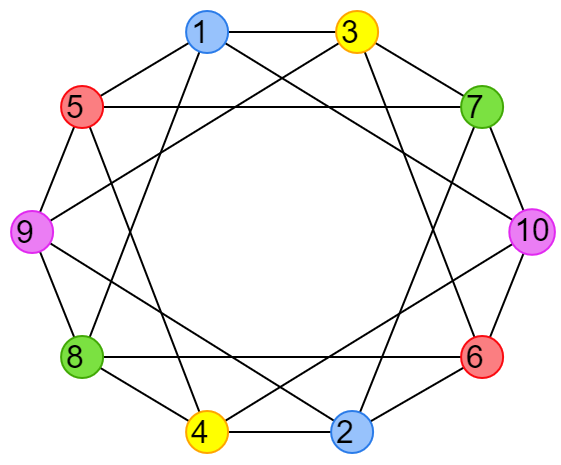
\includegraphics[scale=0.40]{graph-5.png}
\caption{Worst-case coloring of \(H\) using either greedy heuristic}
\end{figure}

\newpage

In Figure 5, using either greedy heuristic with this ordering, we get \(\chi(H) = 5\). This gives us \(\frac{|V|}{2}\) colors. This is the worst-case for a crown graph, but this graph also demonstrates the upper bounds for these greedy algorithms. \newline

\subsection*{In General}

Let \(P = (V, E)\) be a simple, complete graph. \newline

We can see that \(\chi(H) = \Delta(H) + 1\). This is very easy to see in a \emph{complete} graph, where all vertices are connected to every other vertex. This means all vertices have degree \(|V| - 1\). Thus, every time we color a node, a new color is needed. And since we have \(\Delta(P) = |V| - 1\) and \(|V|\) vertices, we will need \(\Delta(P) + 1\) colors. This is proved in \emph{Brooks' Theorem}.

\begin{theorem}[Brooks' Theorem]
For any connected undirected graph \(G\) with maximum degree \(\Delta\), the chromatic number of \(G\) is at most \(\Delta\) unless \(G\) is a complete graph or an odd cycle, in which case the chromatic number is \(\Delta + 1\).
\end{theorem}

Overall, the greedy and the greedy plus degree sequencing heuristics can produce some very bad results. In graph \(H\), at the worst case, the greedy heuristic produces \(\chi(H) = 5\) when \(\chi^{*}(H) = 2\) as it is bipartite. This is shown below.

\begin{figure}[H]
\centering
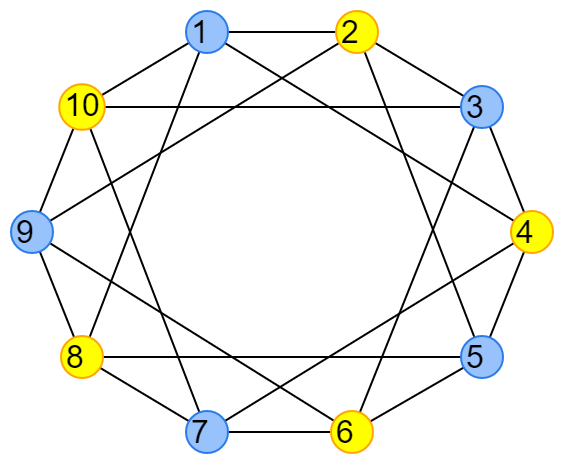
\includegraphics[scale=0.40]{graph-6.png}
\caption{Optimal coloring of \(H\)}
\end{figure}


\end{document}
